\documentclass[letterpaper,twocolumn]{article}

\usepackage{graphicx}

\usepackage[dvips,pdftex]{hyperref}

\usepackage{listings}
\usepackage{color}

\definecolor{mygreen}{rgb}{0,0.6,0}
\definecolor{mygray}{rgb}{0.5,0.5,0.5}
\definecolor{mymauve}{rgb}{0.58,0,0.82}

\lstset{ %
  backgroundcolor=\color{white},   % choose the background color; you must add \usepackage{color} or \usepackage{xcolor}
  basicstyle=\footnotesize,        % the size of the fonts that are used for the code
  breakatwhitespace=false,         % sets if automatic breaks should only happen at whitespace
  breaklines=true,                 % sets automatic line breaking                    % sets the caption-position to bottom
  commentstyle=\color{mygreen},    % comment style
  deletekeywords={...},            % if you want to delete keywords from the given language
  escapeinside={\%*}{*)},          % if you want to add LaTeX within your code
  extendedchars=true,              % lets you use non-ASCII characters; for 8-bits encodings only, does not work with UTF-8
  frame=single,                    % adds a frame around the code
  keepspaces=true,                 % keeps spaces in text, useful for keeping indentation of code (possibly needs columns=flexible)
  keywordstyle=\color{blue},       % keyword style
  language=Octave,                 % the language of the code
  morekeywords={*,...},            % if you want to add more keywords to the set
  numbers=left,                    % where to put the line-numbers; possible values are (none, left, right)
  numbersep=5pt,                   % how far the line-numbers are from the code
  numberstyle=\tiny\color{mygray}, % the style that is used for the line-numbers
  rulecolor=\color{black},         % if not set, the frame-color may be changed on line-breaks within not-black text (e.g. comments (green here))
  showspaces=false,                % show spaces everywhere adding particular underscores; it overrides 'showstringspaces'
  showstringspaces=false,          % underline spaces within strings only
  showtabs=false,                  % show tabs within strings adding particular underscores
  stepnumber=2,                    % the step between two line-numbers. If it's 1, each line will be numbered
  stringstyle=\color{mymauve},     % string literal style
  tabsize=2,                       % sets default tabsize to 2 spaces
  title=\lstname                   % show the filename of files included with \lstinputlisting; also try caption instead of title
}

\lstdefinestyle{customasm}{
  belowcaptionskip=1\baselineskip,
  frame=L,
  xleftmargin=\parindent,
  language=[x86masm]Assembler,
  basicstyle=\footnotesize\ttfamily,
  commentstyle=\itshape\color{purple},
}
\lstset{language=C}

\author{Luke Fraser}
\title{Programming Assignment One}
\date{\today}

\begin{document}
\maketitle

\begin{abstract}
In this assignment we implemented GPU accelerated vector addition use the CUDA programming language. This is an intro into GPU computing assignment designed to provide a basic knowledge of how programming in CUDA works. We look into efficient memory access with striding and compare to non-strided versions of vector addition. As well a comparison of a CPU implementation vs. a GPU implementation is performed to understand the benefits of running parallel processes on the GPU.
\end{abstract}

\section{Introduction}
General purpose GPU computing has a lot to offer as far as computing power is concerned and in many cases is left untapped on a system. Traditional computational problems that lend themselves to parallelism can be accelerated on the GPU. In many cases the GPU can outperform the CPU. This provides a big incentive to run large computations on the GPU over the CPU. Higher throughput can be achieved so that more data can be processed over the CPU.

In this assignment vector addition was run on the CPU and GPU to show the differences in runtime. As well the CUDA language was used to communicate with an NVIDIA GTX 750 video card. The GTX 750 has 512 CUDA cores and supports the 5.0 standard of the CUDA language.

\begin{table*}
\centering
\begin{tabular}[c]{|l|l|l|l|l|} \hline
Elements & No Stride Mean & No Stride Std. Dev. & Stride Mean & Stride Std. Dev.\\ \hline
1,000,000 & 2.592980096 & 0.3607263888 & 2.351109824 & 0.2748393532\\ \hline
10,000,000 & 27.005150314 & 5.1449789588 & 17.360746746 & 1.6349493497\\ \hline
100,000,000 & 350.736235364 & 35.0031726612 & 169.664086342 & 4.6850383716 \\ \hline
\end{tabular}
\caption{Execution time mean and standard deviation}
\label{tab:exec}
\end{table*}

\section{GPU Vector Addition}
Using the CUDA language vector addition was programmed to run the GTX 750 video card. The CUDA language uses several mechanisms to contorl the way an algorithm is run on the video card.CUDA presents you with Grids, Blocks, and Threads.
\subsection{Grids}
Grids are an item on the video card that contain a number of Blocks. Girds can be registered in 3 dimensional format with an x,y,z component.
\subsection{Blocks}
Blocks are an item in CUDA that are contained within a Grid and contain a number of threads. Each Block can have a number of Threads assigned to it. Blocks like Grids can also be registered in a 3 dimensional format with an x,y,z component.
\subsection{Threads}
Threads are contained within Blocks and there are so many Threads run per Block. A single Thread will run a kernel of CUDA code. In the case of vector addition a thread can be thought to perform a single element of the addition. so if there were 1024 elements to be added a single thread per element could be spawned to simultaneously add each element of the vectors. This would allow for a massive speedup over a sequential execution where each element has to added one after the other.
\subsection{Implementation}
\begin{table}
\centering
\begin{tabular}[t]{|l|l|l|} \hline
Speedup CPU & No Stride & Stride\\ \hline
1,000,000 & 1.3923105718 & 1.5355444323\\ \hline
10,000,000 & 1.1945520993 & 1.8581607964\\ \hline
100,000,000 & 0.8886057144 & 1.8369604889 \\ \hline
\end{tabular}
\caption{Speedup Factor over Core i7 Ivy Bridge roughly 3.3GHz}
\end{table}
In the case of the program developed for this assignment the CUDA kernel was not designed in such a way that forced a single thread to operate on a single element of a vector. The program allowed for an arbitrary number of blocks to be generated as well as a arbitrary number of threads per block to be spawned. Each of these numbers could be passes as parameters to the program. Three implementations of vector addition were written: a no memory stride GPU version, a memory striding version, and a CPU version. Each were run many time against with different parameters and compared against each other. In the case of the CPU version on the number of elements in the vectors could be changed as a parallel implementation was not written.
\subsection{Striding}
Striding was used to improve memory access performance on the GPU. The goal being that instead of loading memory from different location each thread would load memory from locations near each other so that the memory fetch would grab all of the data at once. My implementation did not adequately stride the data and a performance improvement was not seen.

\section{Results}

The program was run 100 times each with different Blocks and threads per block passed as parameters to generate the graphs below. Each Block and Thread per block pair was samples 5 times to achieve an average runtime for the data set. These average were plotted to produce the figures~\ref{fig:1million},~\ref{fig:10million},~\ref{fig:100million}.
\begin{figure}
 \centering
 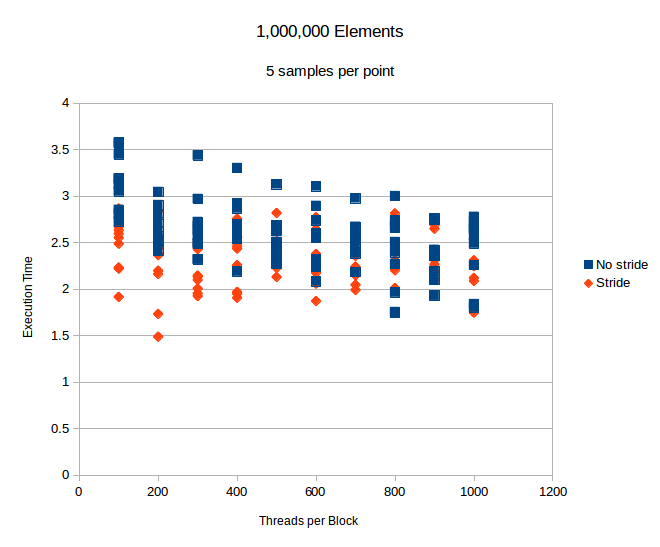
\includegraphics[width=8cm]{1000000_graph.png}
 \caption{1 million element vector addition runtime graph.}
 \label{fig:1million}
\end{figure}
When only a million elements were sent to the GPU for computing the difference between strided and non-strided access was less pronounced as can be seen in figure~\ref{fig:1million}. As well the standard deviation of the two sets is similar. As both the blocks and threads per blocks are changed the runtime gets better and worse. A general trend as the blocks increase and the threads per block increase better performance is noticed. This improvement is not very pronounced.

\begin{figure}
 \centering
 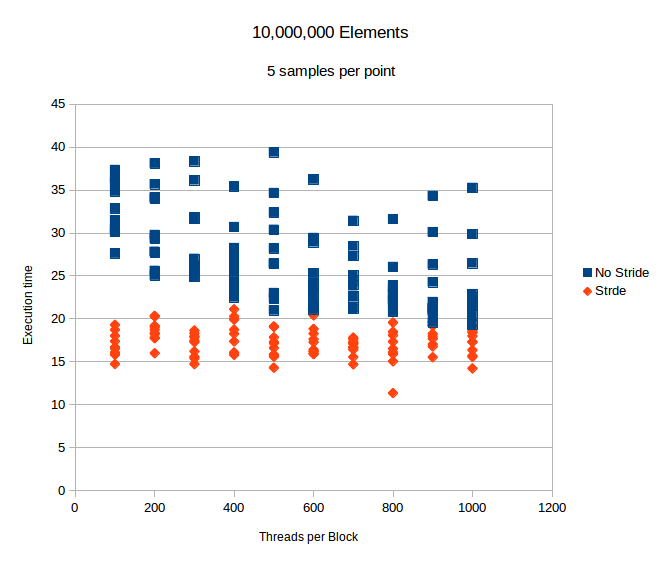
\includegraphics[width=8cm]{10,000,000_graph.png}
 \caption{10 million element vector addition runtime graph.}
 \label{fig:10million}
\end{figure}
As the number of elements increases a greater trend in performance is noticed on the GTX 750 as seen in figure~\ref{fig:10million}. Clearly striding out performs the non-striding schema and the standard deviation is much more tightly bound around the strided run-times. This trend is even more clear in the 100 million element case as seen in figure~\ref{fig:100million}. It is very apparent that memory access is one of the most important aspects at achieving a stable runtime with different block and thread per block sizes. The non-strided kernel even at 100 million still varies wildly across different block and kernel sizes. This result makes sense due to the fact that memory access is such a slow operation overall and without proper memory access techniques getting reliable performance is simply impossible.

\begin{figure}
 \centering
 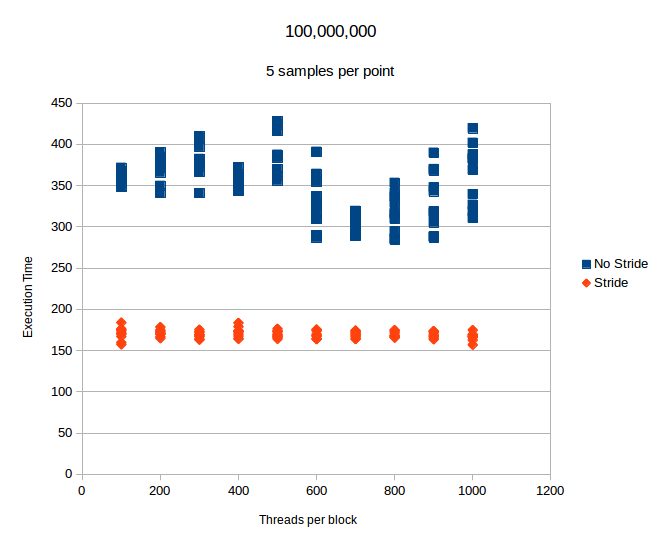
\includegraphics[width=8cm]{100,000,000_graph.png}
 \caption{100 million element vector addition runtime graph.}
 \label{fig:100million}
\end{figure}

\begin{figure*}
\begin{lstlisting}
__global__ void add_no_stride(int *a, int *b, int *c, int elements_per_thread) {
  int offset = blockIdx.x * blockDim.x * elements_per_thread + threadIdx.x * elements_per_thread;
  for (int i = 0; i < elements_per_thread; ++i) {
    c[offset + i] = a[offset + i] + b[offset + i];
  }
}
\end{lstlisting}
\caption{CUDA vector add: No Stride}
\label{fig:nostride}
\end{figure*}

\begin{figure*}
\begin{lstlisting}
__global__ void add_stride(int *a, int *b, int *c, int elements_per_thread) {
  int offset = blockIdx.x * blockDim.x * elements_per_thread + threadIdx.x;
  for (int i = 0; i < elements_per_thread; ++i) {
    c[offset + i * blockDim.x] = a[offset + i * blockDim.x] + b[offset + i * blockDim.x];
  }
}
\end{lstlisting}
\caption{CUDA vector add: Stride}
\label{fig:stride}
\end{figure*}
\section{Discussion}
Due to the complex CUDA kernel functions I wrote I believe this is cause for concern with the lack of large scale speedup. If the kernels didn't have for-loops and large offset calculations I believe the speedup factor would be much larger.
\end{document}
